
\begin{section}{Simulation Results}
\label{sec:simulation}

% Need to label states of the state vector in the modeling section [x y v \theta]

The case study investigated in this paper is with a ground vehicle experiencing the effects of sensor and process noise, dynamical changes, while also succumbing to wind disturbances and sensor attacks. The vehicle will be traveling along a pre-planned trajectory with assumed to be known obstacles throughout the environment. We consider a ground vehicle starting at an initial position $\bm{p}(0)=\begin{bmatrix} 22,10 \end{bmatrix}^T$ facing the positive $x$ direction with zero velocity. The objective for the vehicle is to reach a goal point while following a desired trajectory with obstacles of varying distances from the path. It is assumed the maximum velocity of the vehicle is 3.0m/s and the desired reference velocity it wants to maintain is 2.5m/s. For simulations...




\begin{figure*}[b!th]
%\begin{figure*}[th!]
\begin{tabular}{cccc}

\subfigure[\label{fig:low_noise} ]{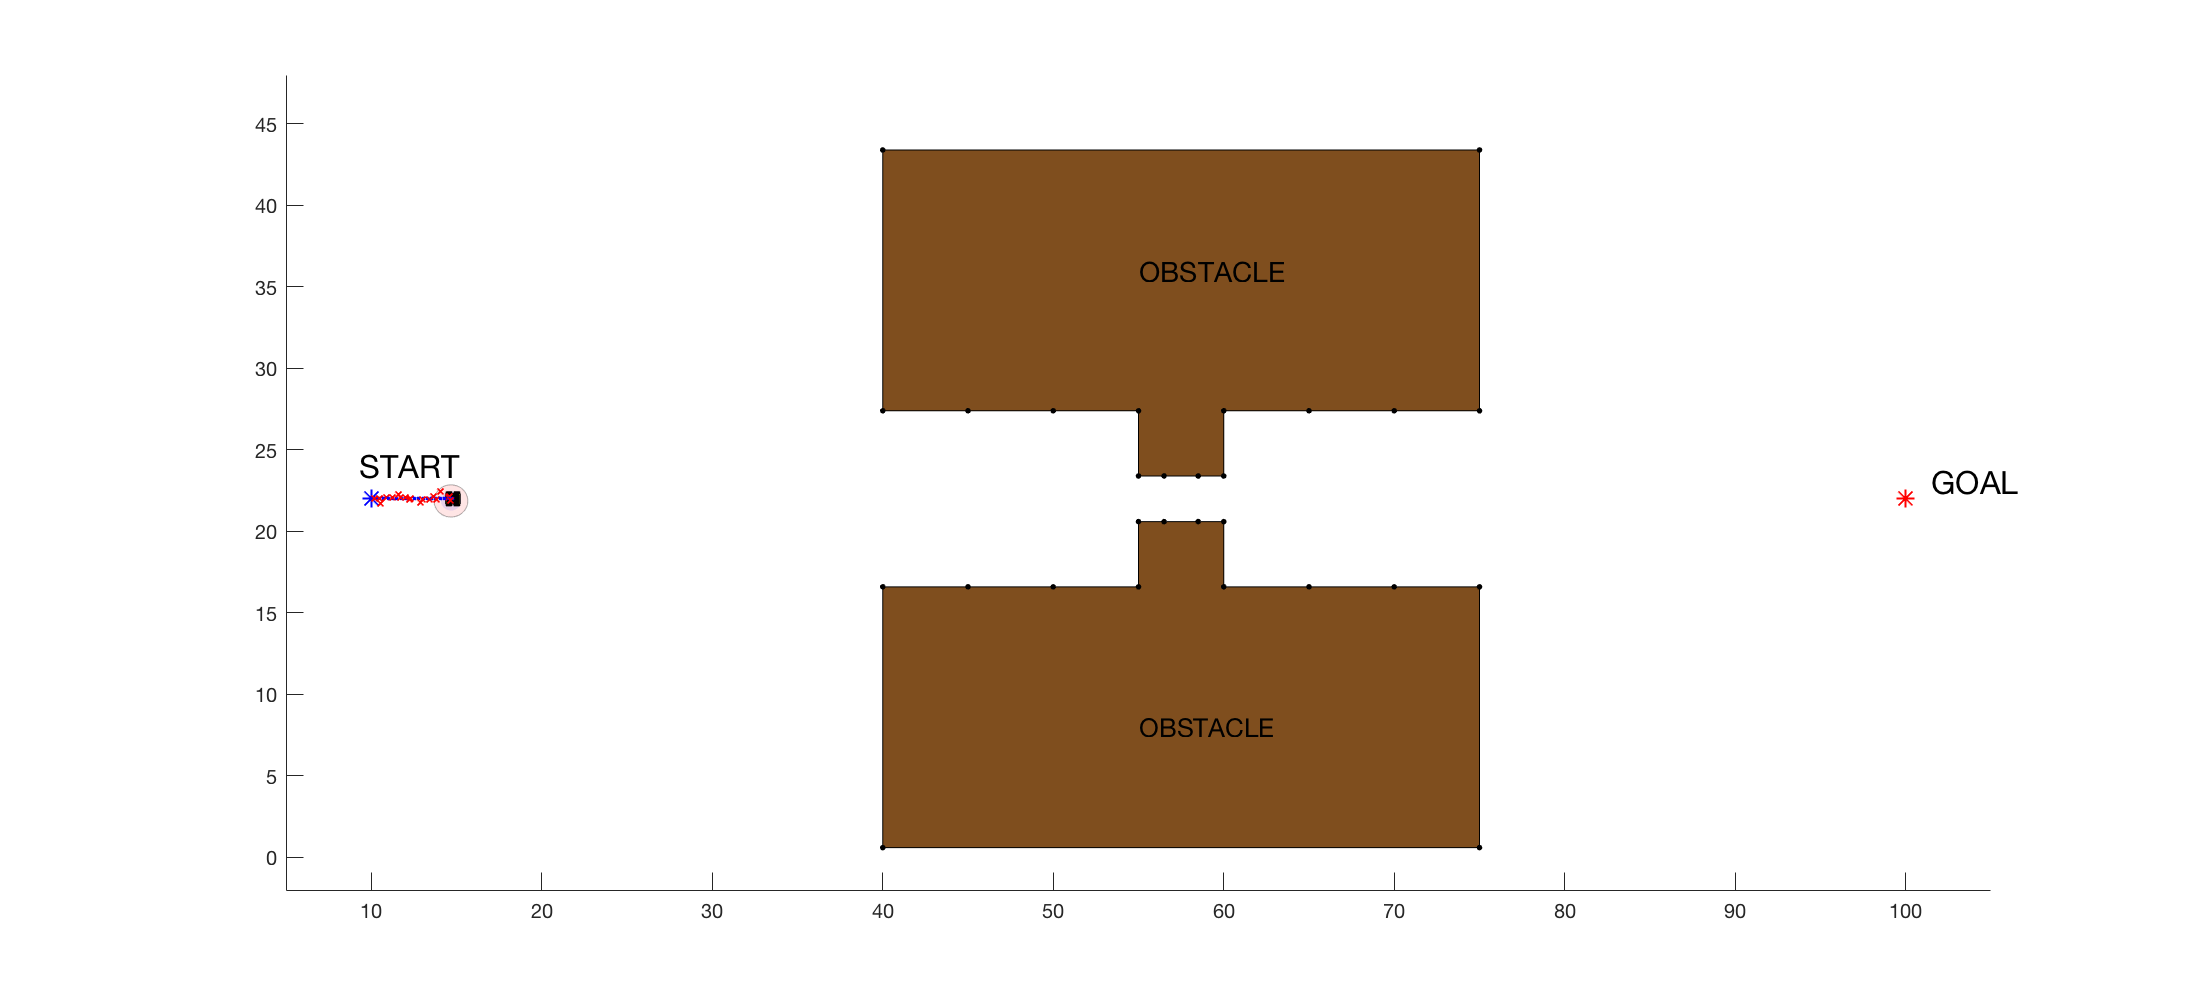
\includegraphics[width = 0.22\textwidth]{Motion1.png}} &	

\subfigure[\label{fig:high_noise} ]{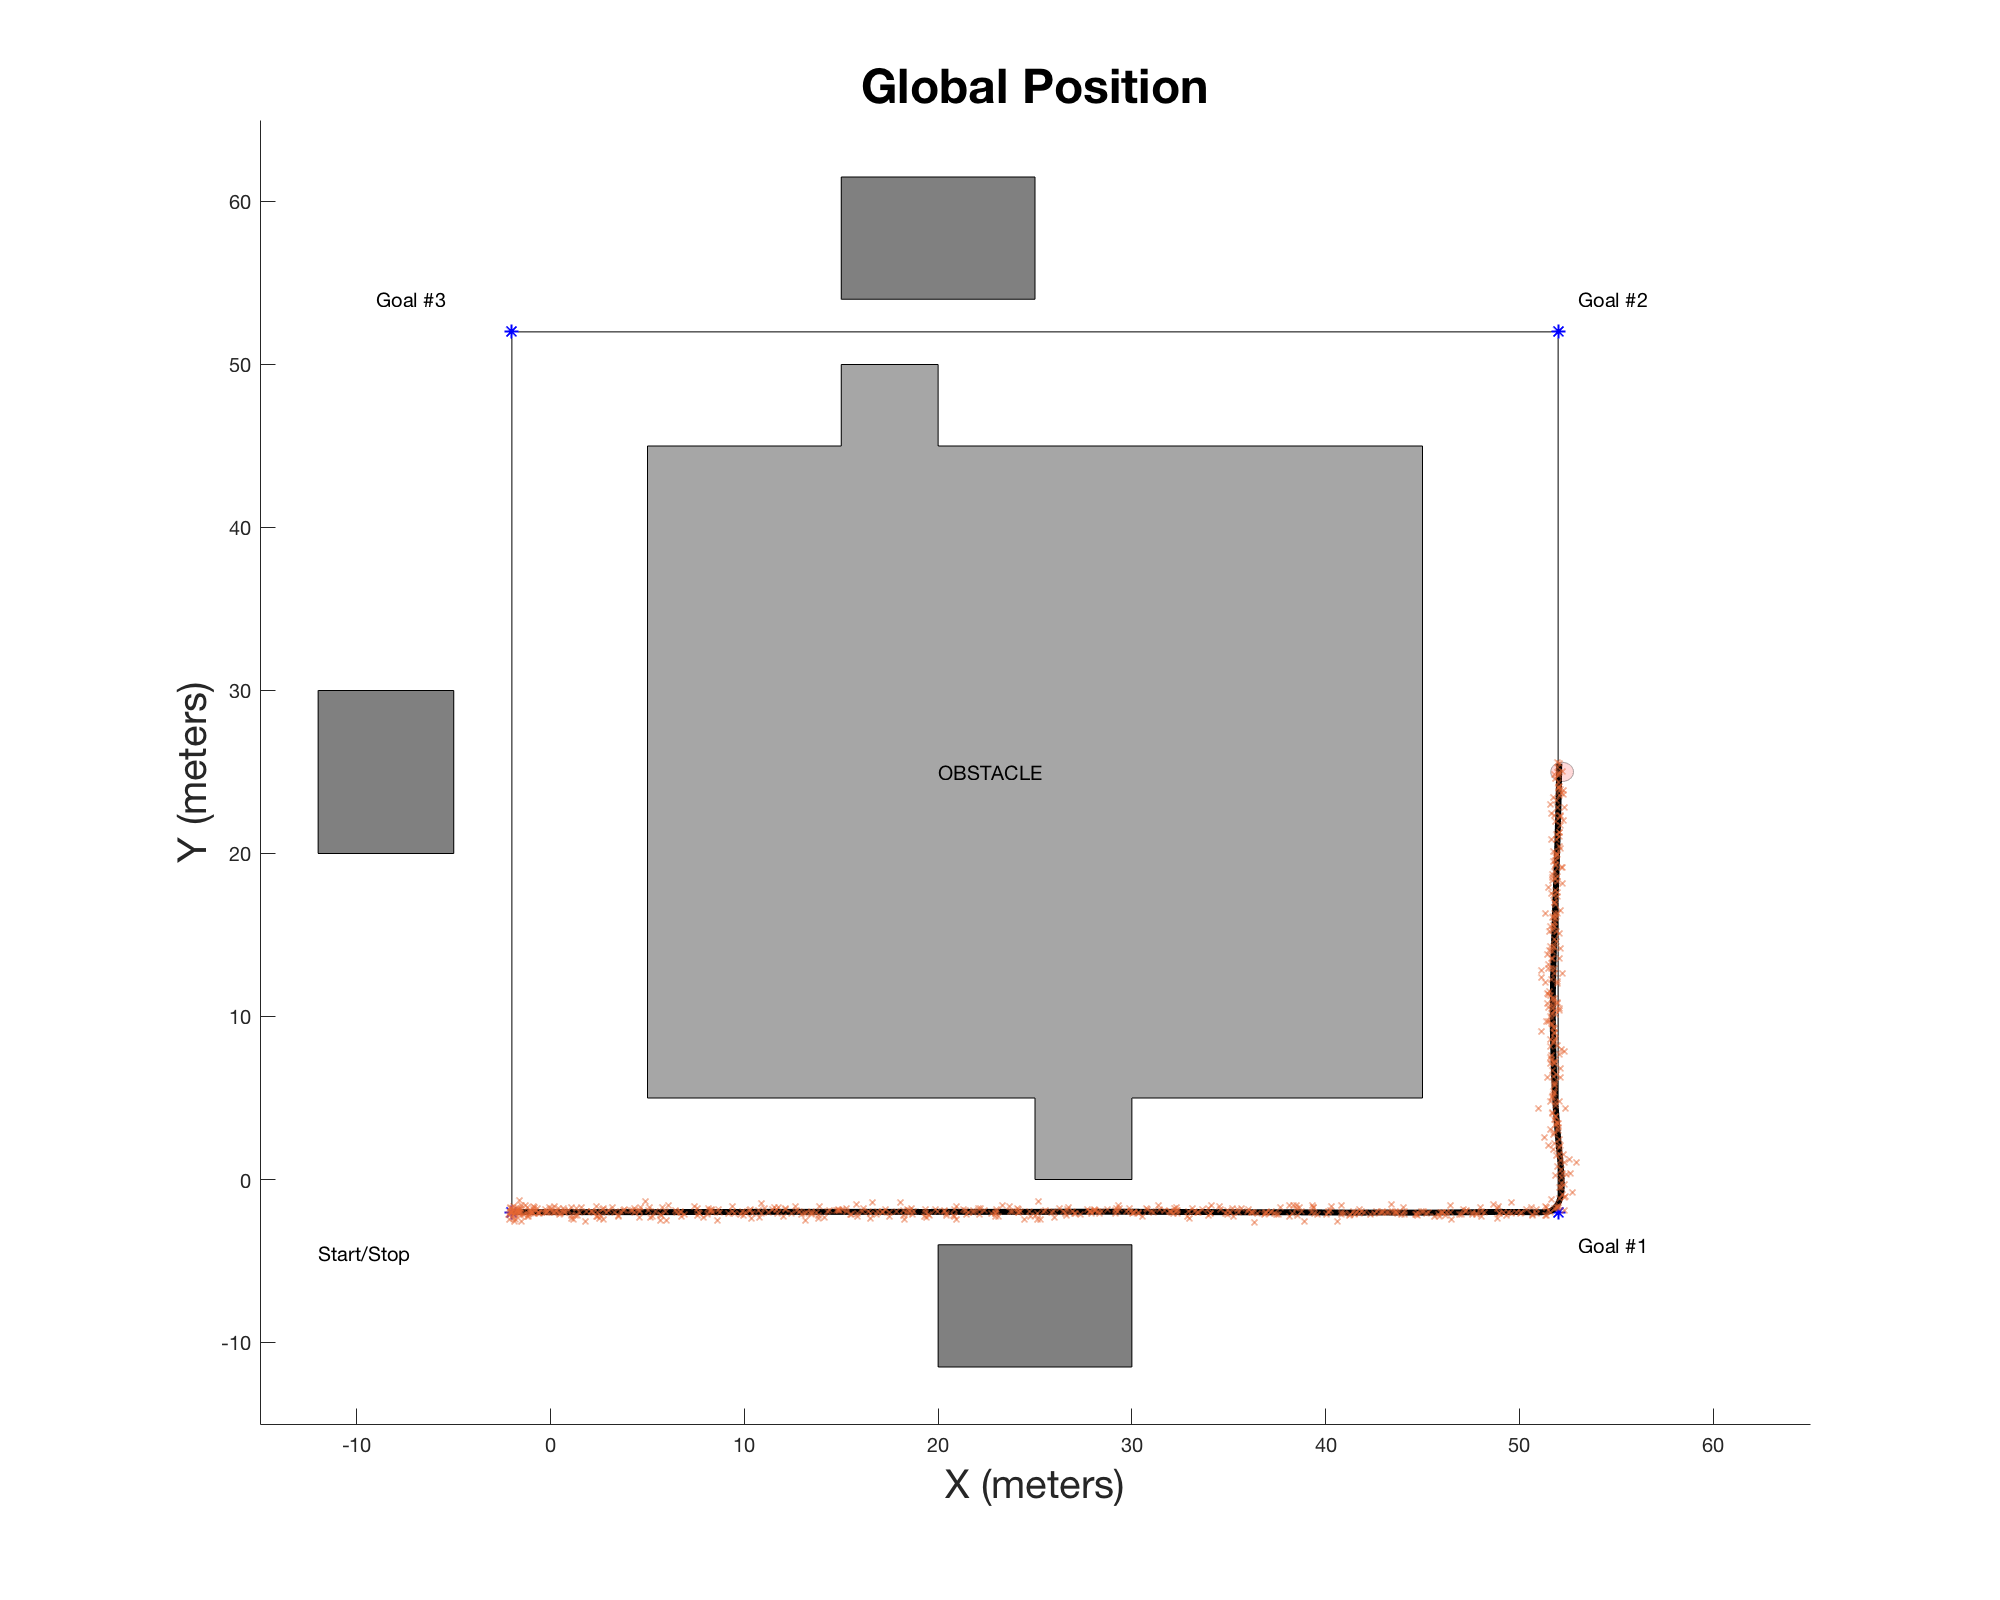
\includegraphics[width = 0.22\textwidth]{Motion2.png}}  &
	
\subfigure[\label{fig:near_obstacle} ]{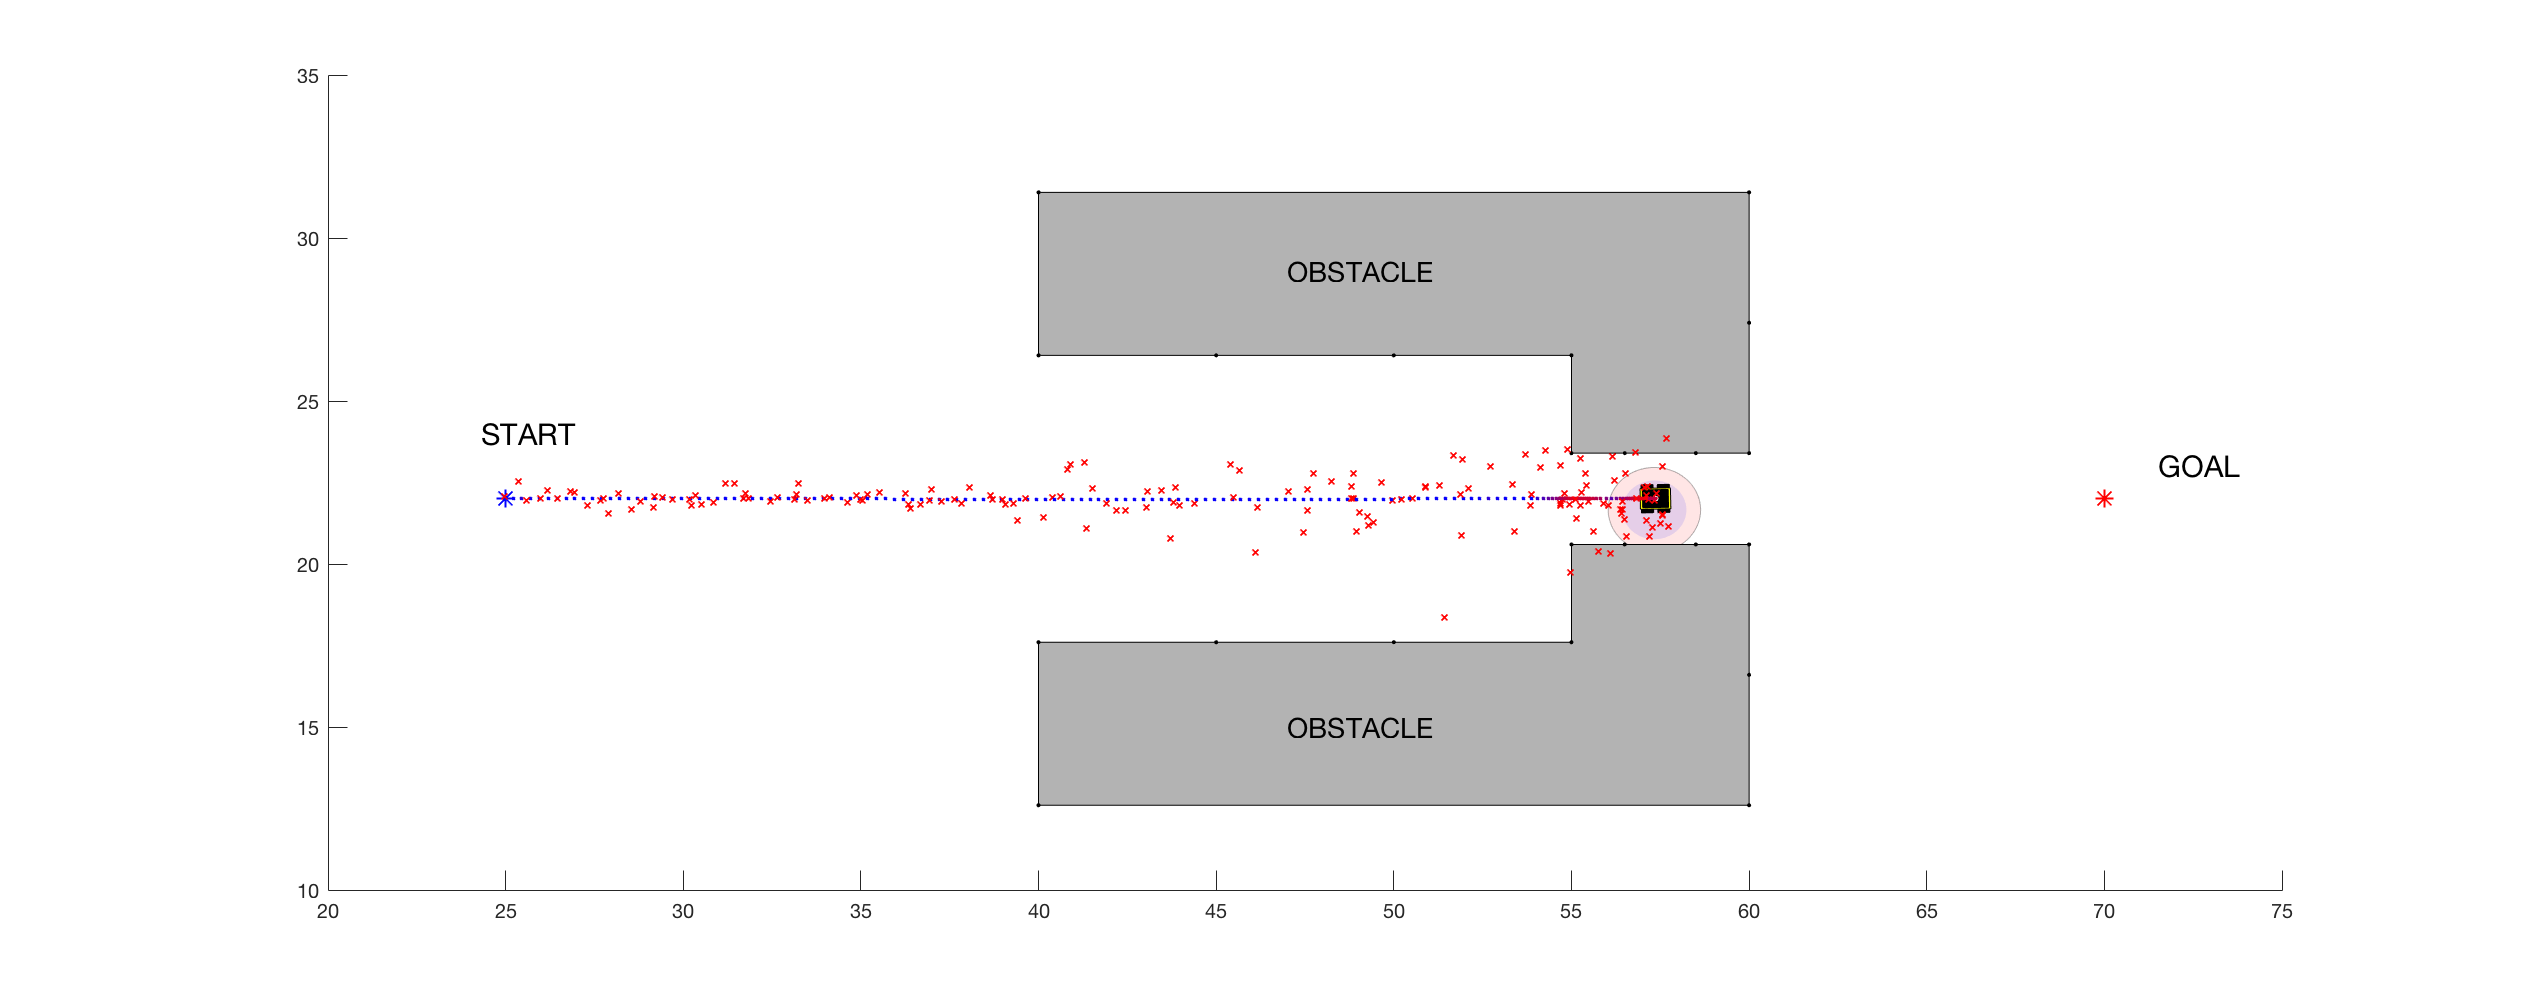
\includegraphics[width = 0.22\textwidth]{Motion3.png}} &

\subfigure[\label{fig:far_obstacle} ]{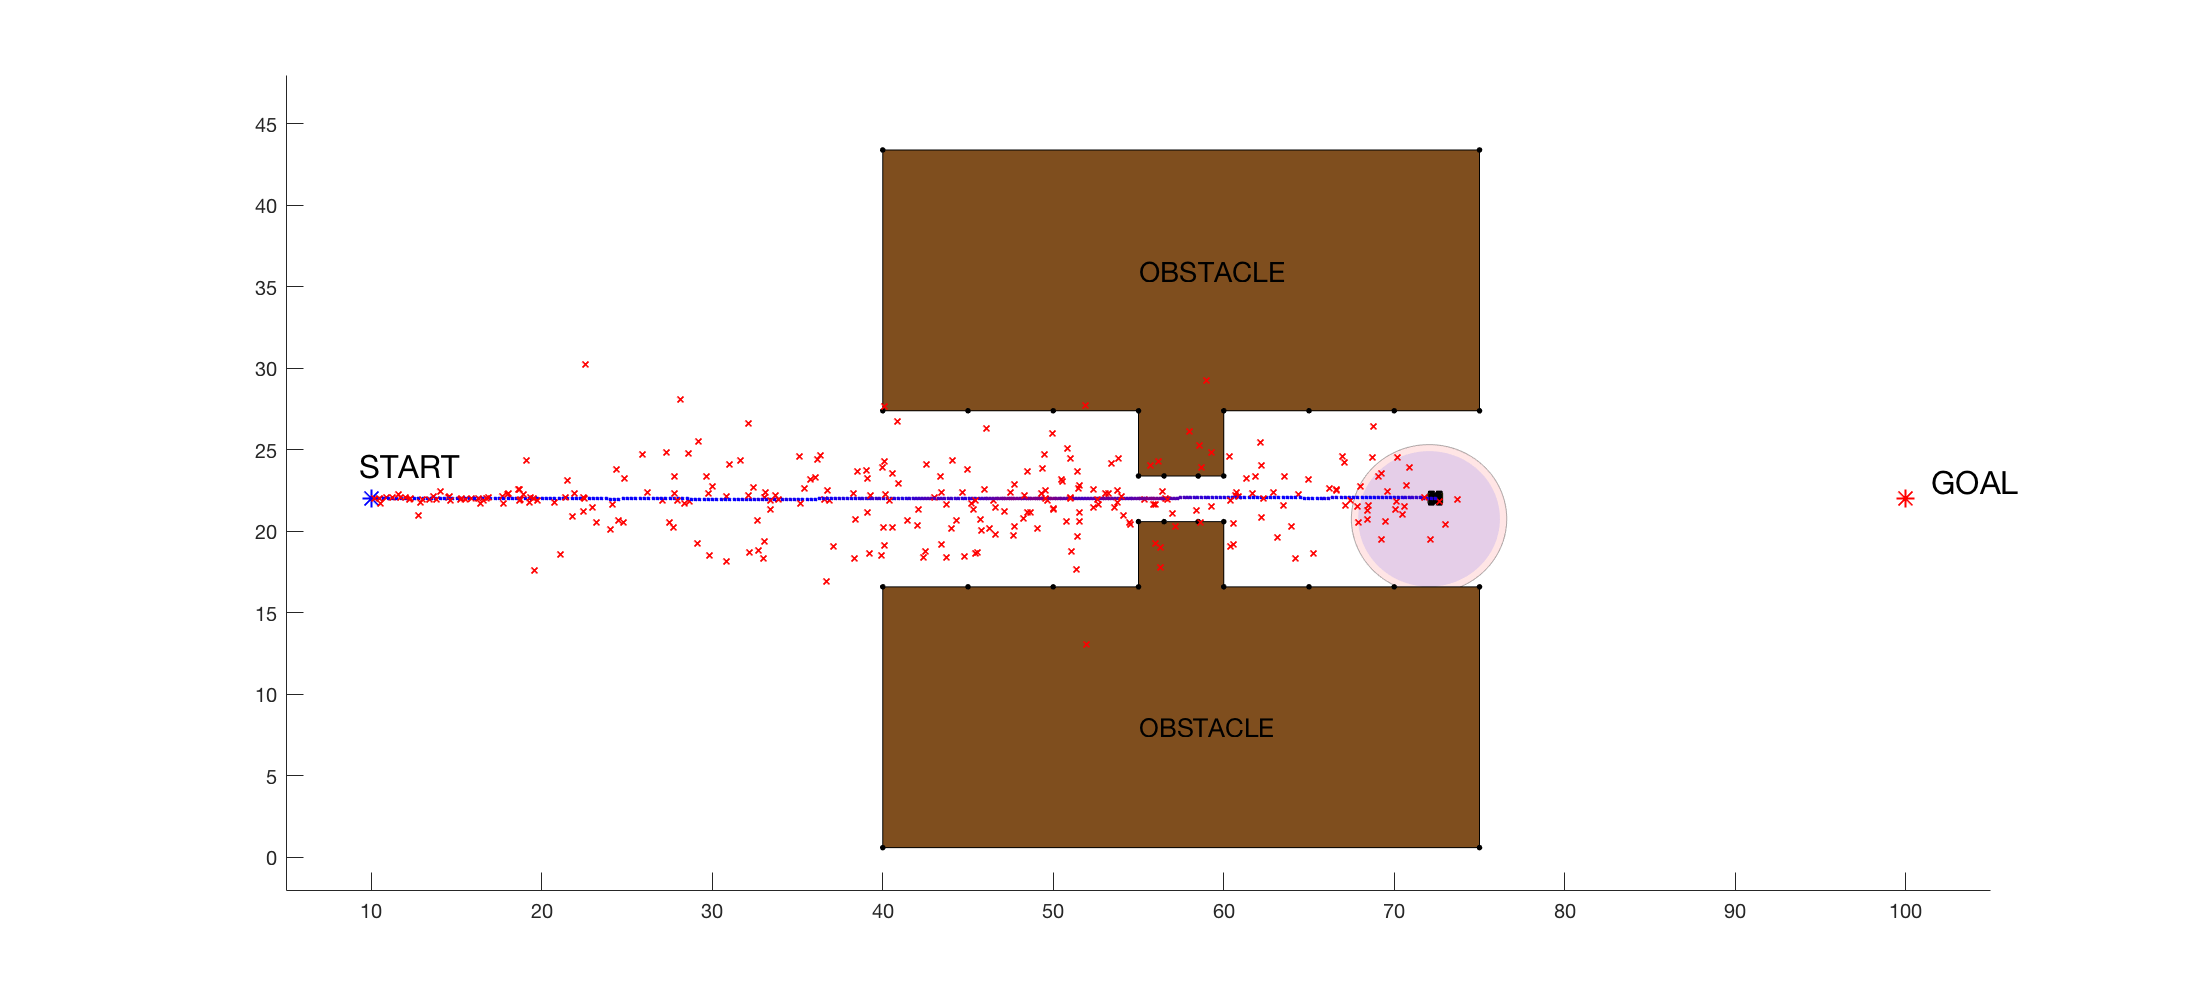
\includegraphics[width = 0.22\textwidth]{Motion4.png}}

\end{tabular}
\caption{A comparison in time of a vehicle navigating through an obstacle filled environment. In (a), the position sensor at this time has low uncertainty, in (b) the original position sensor has been removed and replaced by a sensor with higher uncertainty, in (c), the confidence region shrinks as more data samples are used and the velocity decreases to guarantee safety of nearby objects and in (d), the obstacles are again far away, so less data samples are needed and the velocity returns to it's desired state. }

\end{figure*}

In Figure \ref{fig:low_noise}, the vehicle moving along the trajectory with no compromised sensors and far from obstacles. The confidence region is, in general, small because the best available sensor with low amount of noise is available . Velocity is unaltered due to the obstacles being well outside the uncertainty boundaries.

Figure \ref{fig:high_noise} demonstrates the effects of the loss of a position sensor of low noise profile due to detection of a sensor attack. A different sensor of higher uncertainty is being used for positional coordinate data. The confidence estimation region has grown in size due to these differing uncertainties.

Figure \ref{fig:near_obstacle} demonstrates the adaptive motion planner in action when obstacles come within the confidence region. More data past samples are used and velocity is decreased to minimize uncertainties for more effective estimation.

In Figure \ref{fig:far_obstacle}, obstacles are again far away from the true position of the vehicle, outside of the confidence region's bounds. Velocity is restored toward desired levels and less data sampled are necessary to remain confident that the vehicle is safe.


FUTURE FIGURES OF ENTIRE SYSTEM AS A WHOLE TO SHOW DETECTION OF ATTACKS (WITH ACTION), DETECTION OF DYNAMICAL CHANGES (WITH NO CORRECTIVE ACTIONS).
Figure Y) displays all sensor measurements for velocity, capturing when the attack occurs and the consequent recovery. 
Figure Z) Showing the detection scheme can decipher the difference between dynamical changes and an attack


\begin{figure}
\vspace{1pt}
\centering
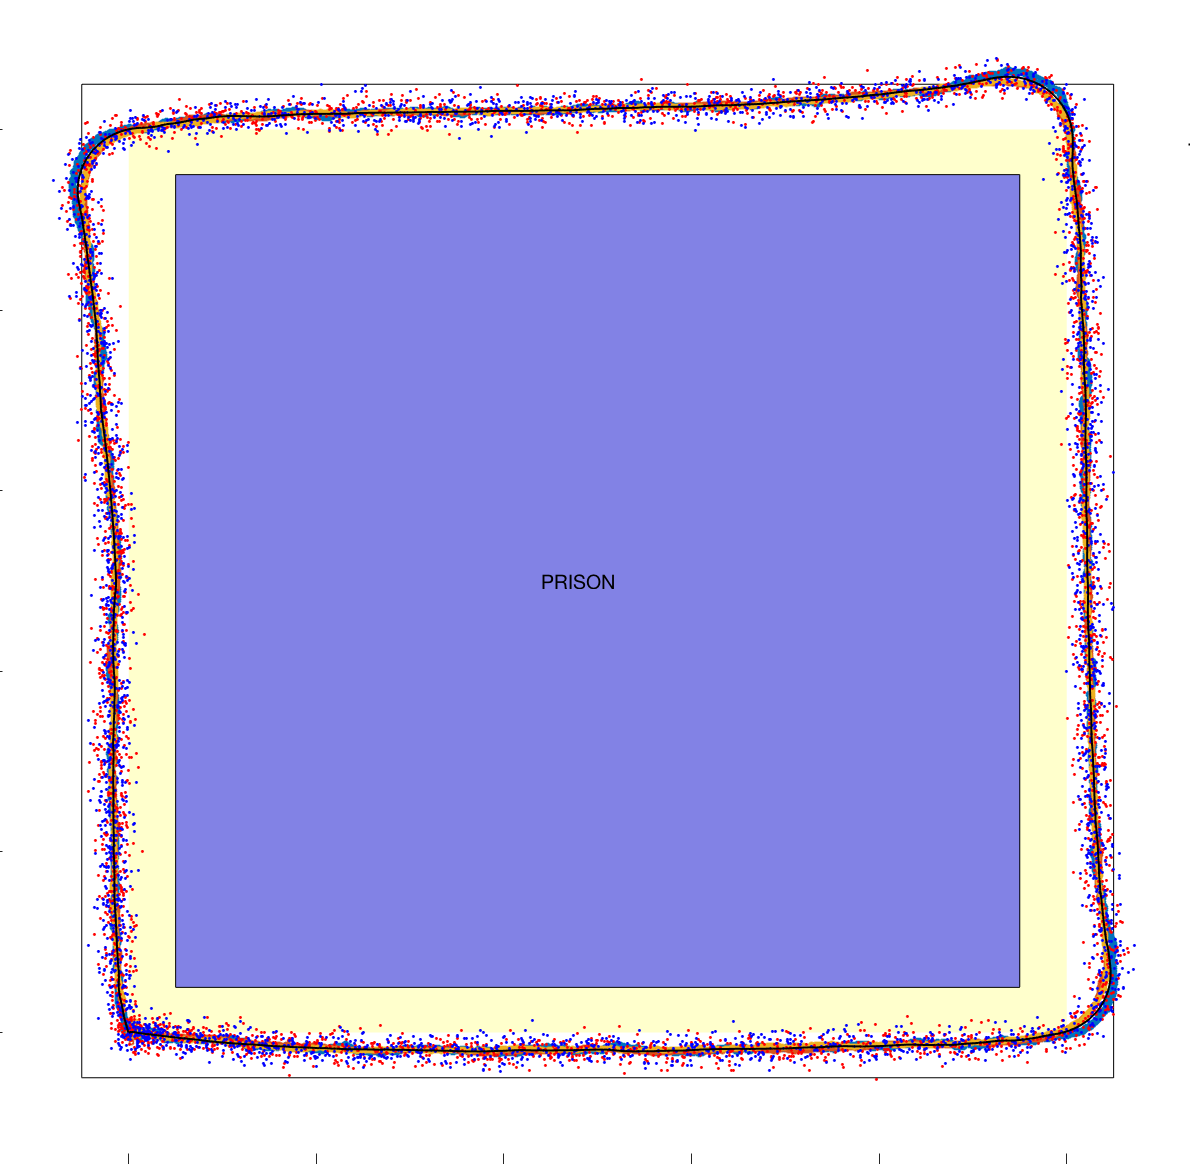
\includegraphics[width=0.48\textwidth]{sim_environment.png}
\caption{The obstacle filled environment the vehicle is traveling through to reach a specified goal point.}
\label{fig:sim_env}
\end{figure}

\begin{figure}
\vspace{1pt}
\centering
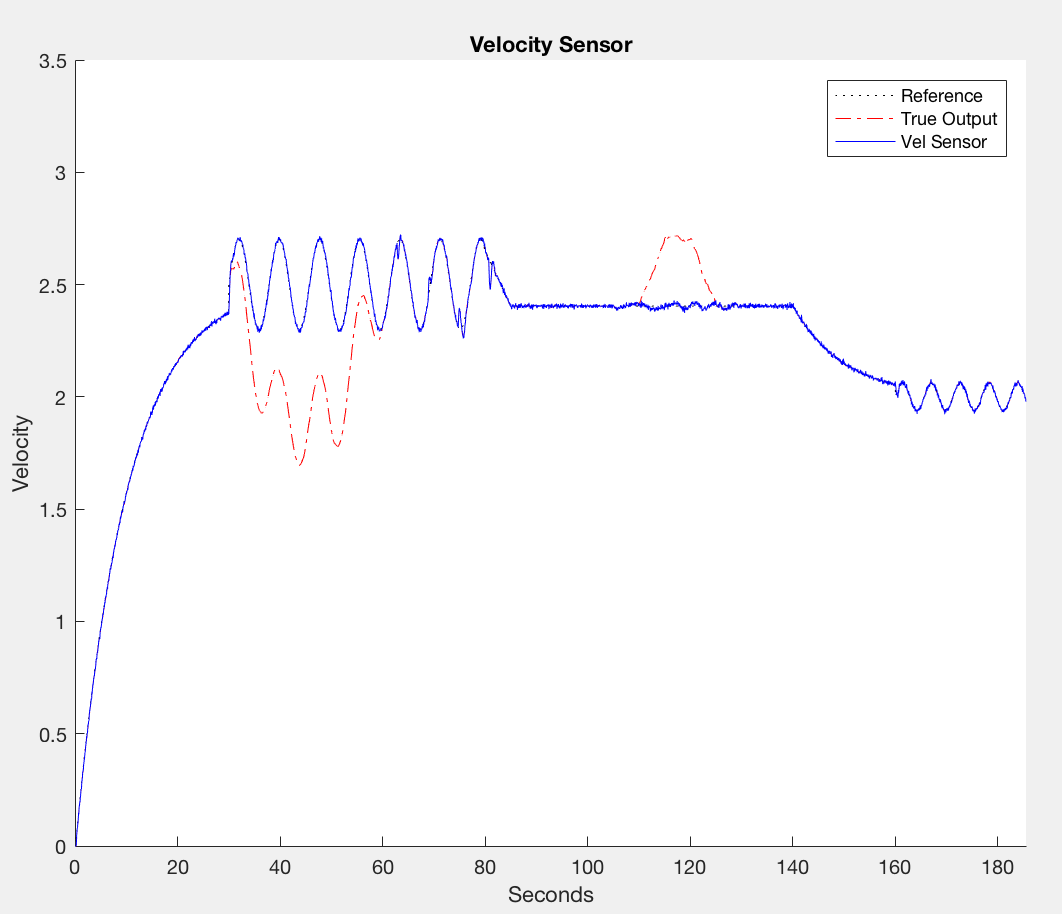
\includegraphics[width=0.48\textwidth]{vel_t.png}
\caption{Vehicle velocity over time exhibiting an attack on a velocity sensor while the system detects and corrects.}
\label{fig:vel_t}
\end{figure}

\begin{figure}
\vspace{1pt}
\centering
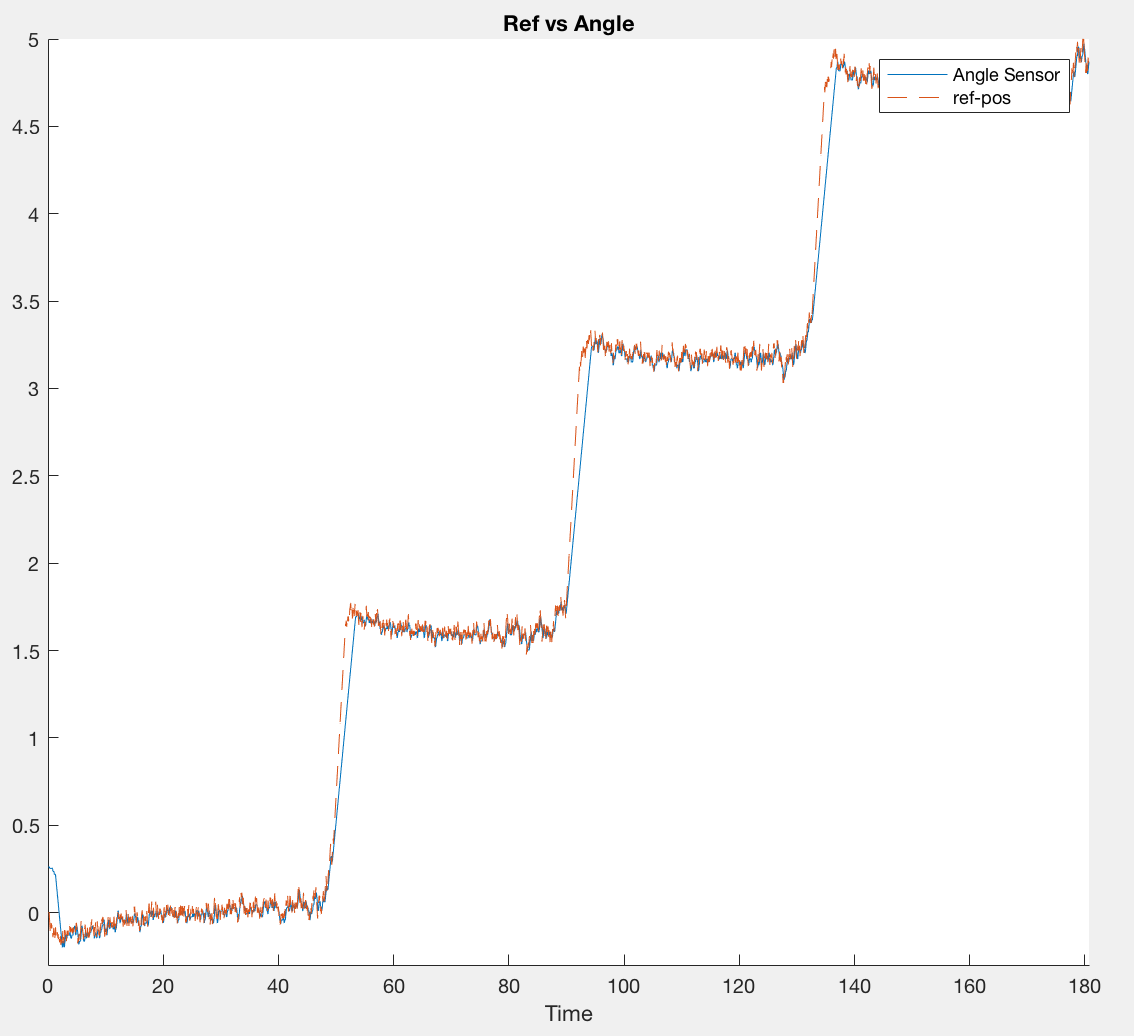
\includegraphics[width=0.48\textwidth]{ang_t.png}
\caption{Vehicle heading angle over time exhibiting an attack on an angle sensor while the system detects and corrects.}
\label{fig:ang_t}
\end{figure}

\end{section}